%= local definitions of macros ============================
\newcommand{\Herwig}{H\protect\scalebox{0.8}{ERWIG}\xspace}
\newcommand{\Pythia}{P\protect\scalebox{0.8}{YTHIA}\xspace}
\newcommand{\Sherpa}{S\protect\scalebox{0.8}{HERPA}\xspace}
\newcommand{\Rivet}{R\protect\scalebox{0.8}{IVET}\xspace}
\newcommand{\Recola}{R\protect\scalebox{0.8}{ECOLA}\xspace}
\newcommand{\Amegic}{A\protect\scalebox{0.8}{MEGIC}\xspace}
\newcommand{\Professor}{P\protect\scalebox{0.8}{ROFESSOR}\xspace}
\newcommand{\OpenLoops}{O\protect\scalebox{0.8}{PENLOOPS 2}\xspace}
\newcommand{\Collier}{C\protect\scalebox{0.8}{OLLIER}\xspace}
\newcommand{\Madgraph}{M\protect\scalebox{0.8}{G5\_aMC@NLO}\xspace}
\newcommand{\eps}{\varepsilon}
\newcommand{\mc}[1]{\mathcal{#1}}
\newcommand{\mr}[1]{\mathrm{#1}}
\newcommand{\mb}[1]{\mathbb{#1}}
\newcommand{\tm}[1]{\scalebox{0.95}{$#1$}}
\newcommand{\vp}{\ensuremath{\vphantom{\int_a^b}}}
\newcommand{\vP}{\ensuremath{\vphantom{\int\limits_a^b}}}

%= title + authors =====================================
\section{NLO QCD and electroweak corrections to off-shell WWW production\protect\footnote{
  S.~Dittmaier,
  G.~Knippen,
  M.~Sch{\"o}nherr,
  C.~Schwan}{}}

%= MANDATORY label ======================================
\label{sec:WWW}

%= (optional) preamble ================================== 

%= intro ===== ==========================================
\subsection{Introduction}
\label{sec:WWW:intro}

Owing to its high scattering energy and luminosity, the LHC is able 
to explore particle processes up to energy scales of several TeV 
even if the corresponding cross sections are in the range of
femtobarns only. 
For the experimental investigation of electroweak (EW) interaction,
this means that the LHC can observe the phenomenologically highly
interesting processes of EW vector-boson scattering (VBS) and
of triple EW vector-boson production (TVP) for the first time.
The analysis of those process classes is particularly interesting
because of their direct sensitivity to quartic gauge self-interations
and to off-shell Higgs-boson exchange. The latter property renders
thoses processes an alternative window to EW symmetry
breaking, complementary to processes with direct (on-shell)
Higgs-boson production.
In this contribution we focus on triple W-boson production, which
was analyzed by ATLAS~\cite{Aaboud:2016ftt,Aad:2019dxu}
and CMS~\cite{CMS:2019mpq} with 4.1$\sigma$ evidence by ATLAS in Run~2.

Taking into account the decays of the EW massive vector bosons,
the VBS and TVP processes are of the types 
$\Pp\Pp\to 4\mathrm{leptons}+2\mathrm{jets}+X$
and $\Pp\Pp\to 6\mathrm{leptons}+X$, respectively, and thus involve
already six particles at leading order (LO).
The calculation of radiative corrections to processes of such complexity is 
rather demanding. 
For TVP processes with leptonically decaying vector bosons, the calculation
of NLO QCD corrections (up to the phase-space integration) has only the complexity
of a $2\to3$ particle process, so that in particular 
the NLO QCD corrections to WWW production with \cite{Campanario:2008yg} 
and without \cite{Binoth:2008kt} leptonic decays have been known for more than ten years.
The NLO EW corrections to WWW production were first calculated for stable W~bosons
and for on-shell W~bosons with decays treated in the narrow-width approximation
in Refs.~\cite{Yong-Bai:2016sal,Dittmaier:2017bnh,Frederix:2018nkq}, before a 
treatment of the full off-shell $2\to6$ process became possible.
This last step poses the challenge of one-loop diagrams with up to eight
particles in the loop (8-point functions), the evaluation of which was
only possible with great advances in the automated calculation of one-loop
amplitudes (see, e.g., Ref.~\cite{Denner:2019vbn} for details and references).

Recently, two independent evaluations of WWW production processes at NLO EW with
leptonically decaying W~bosons, including all off-shell effects, have been
presented in the literature: 
the calculation of Ref.~\cite{Schonherr:2018jva} based on \Sherpa~\cite{Bothmann:2019yzt}
with \Recola~1.2 \cite{Actis:2012qn,Actis:2016mpe} as one-loop matrix element provider 
on the one hand and the two more process-specific calculations of 
Ref.~\cite{Dittmaier:2019twg} based on
\OpenLoops~\cite{Cascioli:2011va,Kallweit:2014xda,Buccioni:2019sur} and 
\Recola~1.4 \cite{Actis:2012qn,Actis:2016mpe} on the other.
Unfortunately, the results of Refs.~\cite{Schonherr:2018jva,Dittmaier:2019twg} initially did not
agree in all parts, rendering a detailed comparison of individual components of the two
calculations necessary.
In this contribution, we briefly report on the methods and tools used in the two calculations,
on the salient features of the NLO corrections, and on the comparison of results that shows good
agreement between the results of Ref.~\cite{Dittmaier:2019twg} and revised results of
Ref.~\cite{Schonherr:2018jva}.


\subsection{Calculational details, methods, and tools}
\label{sec:WWW:methods}

In detail, the NLO calculation of Ref.~\cite{Schonherr:2018jva} for WWW production
employs a combination of \Sherpa 
\cite{Bothmann:2019yzt,Gleisberg:2008ta,Bothmann:2016nao,Hoeche:2014rya} 
and \Recola \cite{Actis:2012qn,Actis:2016mpe}, where
\Sherpa provides the tree-level matrix elements, 
infrared substraction, process management, and phase-space 
integration through its matrix element generator \Amegic 
\cite{Krauss:2001iv,Gleisberg:2007md,Schonherr:2017qcj}. 
\Recola is interfaced \cite{Biedermann:2017yoi} to provide 
all renormalised virtual corrections, where the loop integrals are evaluated with the
\Collier library~\cite{Denner:2016kdg},
which in turn is based on the results of 
Refs.~\cite{Denner:2002ii,Denner:2005nn,Denner:2010tr}.

On the other hand, the results of Ref.~\cite{Dittmaier:2019twg}, called DKS in the following,
were produced and double-checked using two private codes: 
The first one was developed specifically for this process, 
and the second one is a generic code that was already used to calculate other EW 
processes~\cite{Ballestrero:2018anz,Denner:2019tmn,Denner:2019zfp}.
The first code uses dipole subtraction as presented in Ref.~\cite{Catani:1996vz} for QCD corrections and 
in Refs.~\cite{Dittmaier:1999mb,Dittmaier:2008md} for EW corrections.
Matrix elements were generated using \Madgraph \cite{Alwall:2014hca} and \Recola,
and the loop integrals were evaulated with \Collier.
The second code is able to use either dipole subtraction as presented in Ref.~\cite{Catani:1996vz} 
for both QCD and EW corrections, the latter using the trivial substitutions for the Casimir operator 
(see, e.g., in Sect~3.2 of Ref.~\cite{Kallweit:2014xda}) or, alternatively, 
the EW dipole subtraction of Refs.~\cite{Dittmaier:1999mb,Dittmaier:2008md} 
as in the first code.
The matrix elements are provided by \OpenLoops \cite{Cascioli:2011va,Kallweit:2014xda,Buccioni:2019sur}, 
which uses \Collier for the evaluation of rank~0 and 1 tensor one-loop integrals.
Both codes use multi-channel Monte Carlo techniques \cite{Hilgart:1992xu,Kleiss:1994qy} for the phase-space integration with phase-space mappings similar to the ones presented in Ref.~\cite{Dittmaier:2002ap}.

Figure~\ref{fig:www-diagrams} illustrates the various types of diagrams
that occur in the calculation of LO and NLO EW contributions to the cross sections of the
WWW production process $\Pp\Pp\rightarrow\Pe^-\bar\nu_{\Pe}\mu^+\nu_\mu\tau^+\nu_\tau+X$.
\begin{figure}
\centering
%\begin{subfigure}[b]{0.33\textwidth}
%\centering
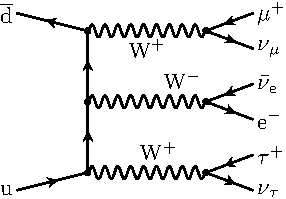
\includegraphics{diagrams/fd02_born_max_t_channel}
%\caption{$t$-channel with 3 resonances}
%\label{fig:triply-res-t-channel}
%\end{subfigure}%
%\begin{subfigure}[b]{0.33\textwidth}
%\centering
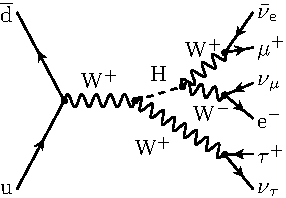
\includegraphics{diagrams/fd03_born_higgs_channel}
%\caption{associated Higgs production}
%\label{fig:associated-higgs-production}
%\end{subfigure}%
%\begin{subfigure}[b]{0.33\textwidth}
%\centering
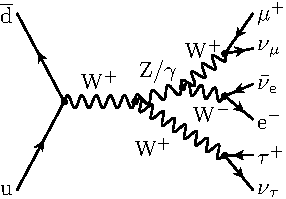
\includegraphics{diagrams/fd04_born_z_channel}
%\caption{$\PW\PZ$ production}
%\label{fig:higgs-replaced-by-z-photon}
%\end{subfigure}%
%\par\bigskip
%\centering
%\begin{subfigure}[b]{0.33\textwidth}
\\[1.5em]
\centering
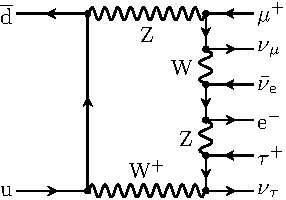
\includegraphics{diagrams/fd12_virtual_8point_box}
%\caption{8-point function}
%\label{fig:nlo-ew-8pt-fun}
%\end{subfigure}%
%\begin{subfigure}[b]{0.33\textwidth}
%\centering
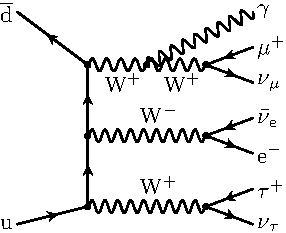
\includegraphics{diagrams/fd09_real_from_w}
%\caption{photon radiation}
%\label{fig:nlo-ew-real}
%\end{subfigure}%
%\begin{subfigure}[b]{0.33\textwidth}
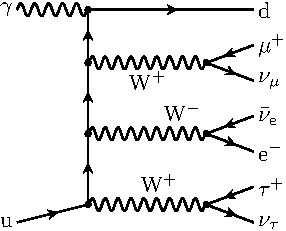
\includegraphics{diagrams/fd14_real_quark_photon}
%\caption{quark--photon induced}
%\label{fig:quark-photon-diagram}
%\end{subfigure}%
\caption{Sample Feynman diagrams contributing to $\Pp\Pp\rightarrow\Pe^-\bar\nu_{\Pe}\mu^+\nu_\mu\tau^+\nu_\tau+X$
at LO (top row) and at NLO EW (bottom row).}
\label{fig:www-diagrams}
\end{figure}
At LO, we can distinguish three basic classes of diagrams acccording to their different resonance structure:
\begin{enumerate}
\item diagrams with three simultaneously resonant \PW bosons (left diagram in the top row of 
Fig.~\ref{fig:www-diagrams}), 
\item Higgs production in association with a \PW boson (middle diagram in the top row of            
Fig.~\ref{fig:www-diagrams}), where the produced Higgs boson further decays into an on- and an off-shell \PW boson, and
\item $\mathrm{WZ}$ production, where the \PZ boson either decays into an on- and an off-shell \PW boson 
(right diagram in the top row of Fig.~\ref{fig:www-diagrams})
or into a four-fermion state via a resonant \PW~boson (not shown in the figure).
\end{enumerate}
All other diagrams show less resonance enhancement.
The production of $\mathrm{WZ}$ is strongly suppressed because of the four-body decay of the \PZ boson, 
while associated Higgs production and triply-resonant $\PW\PW\PW$ contributions dominate the 
cross sections of the given processes.
Due to the extremely narrow width of the Higgs boson and the fact that the Higgs-boson mass is smaller 
than twice the \PW-boson mass, associated Higgs production is well separated from the triply-resonant 
WWW contributions in phase space and therefore can, in principle, be isolated by phase-space cuts.

The bottom row of Fig.~\ref{fig:www-diagrams} shows representative diagrams for the three contributions to
the NLO EW corrections: one-loop contributions (left), photonic bremsstrahlung contributions (middle),
and contributions from photon-induced channels (right). 
Note that both the evaluation of virtual and real corrections is technically challenging,
the former in view of a fast and numerically stable evaluation of loop diagrams up to
8-point complexity, the latter owing to the complicated resonance structures in the 7-particle
phase space.
We finally mention that in all the calculations presented in
Refs.~\cite{Schonherr:2018jva,Dittmaier:2019twg} the resonances are treated in the 
complex-mass scheme \cite{Denner:2005fg} (see also \Ref.~\cite{Denner:2019vbn}),
i.e.\ complex gauge-boson masses defined by 
\begin{equation}
  \mu_V^2=M_V^2-\mathrm{i}M_V\Gamma_V, \qquad V=\PW,\PZ,
\end{equation}
are used in all propagators and couplings consistently, in order to ensure
gauge independence and NLO precision in resonant and non-resonant phase-space regions.

\subsection{Tuned comparison of results from the different NLO calculations}
\label{sec:WWW:comparison}

To compare the independent
calculations laid out in the previous section we 
choose the following setup.
The fiducial cross section for the process 
$\Pp\Pp\rightarrow\Pe^-\bar\nu_{\Pe}\mu^+\nu_\mu\tau^+\nu_\tau+X$
and its charge conjugate counterpart is defined by the phase-space cuts 
on the charged leptons summarized in Tab.~\ref{tab:WWW:cuts}.
\begin{table}[t!]
  \centering
  \begin{tabular}{c|c}
    Kinematical variable & fiducial range\\\hline
    $p_\mathrm{T}(\ell)$ & $[20,\infty]\,\text{GeV}$ \\
    $\eta(\ell)$ & $[-2.5,2.5]$ \\
    $p_\mathrm{T}(\ell_1)$ & $[27,\infty]\,\text{GeV}$ \\
    $\Delta R(\ell_i,\ell_j)$ & $[0.1,\infty]$
  \end{tabular}
  \caption{
    Definition of the fiducial region. Lepton requirements relate 
    to dressed leptons using a cone algorithm with $\Delta R_\text{dress}=0.1$.
    \label{tab:WWW:cuts}
  }
\end{table}
The gauge-boson masses and widths are defined by their on-shell 
values provided by the Particle Data Group \cite{Tanabashi:2018oca}, 
\begin{center}
  \begin{tabular}{ll}
    $M_{\PW}^\text{OS}=80.379\,\text{GeV}$,\qquad & $\Gamma_{\PW}^\text{OS}=2.085\,\text{GeV}$, \\
    $M_{\PZ}^\text{OS}=91.1876\,\text{GeV}$,\qquad & $\Gamma_{\PZ}^\text{OS}=2.4952\,\text{GeV}$.
  \end{tabular}
\end{center}
They are then converted to pole masses using 
\begin{equation}
  M_V=\frac{M_V^\text{OS}}{\sqrt{1+\left(\frac{\Gamma_V^\text{OS}}{M_V^\text{OS}}\right)^2}}\;,
  \qquad
  \Gamma_V=\frac{\Gamma_V^\text{OS}}{\sqrt{1+\left(\frac{\Gamma_V^\text{OS}}{M_V^\text{OS}}\right)^2}}.
\end{equation}
In addition, we set the Higgs-boson and top-quark masses
and widths to 
\begin{center}
  \begin{tabular}{ll}
    $M_{\PH}=125\,\text{GeV}$, & $\Gamma_{\PH}=0.004088\,\text{GeV}$, \\
    $M_{\mathrm{t}}=173\,\text{GeV}$, & $\Gamma_{\mathrm{t}}=0$\;. \\
  \end{tabular}
\end{center}
All remaining quarks and leptons, in particular the bottom quark and the $\tau$-lepton,
are considered massless.
The CKM matrix is parametrised using the Cabibbo angle 
\begin{equation}
  \theta_\text{C}=0.22731\;,\nonumber
\end{equation}
neglecting mixing with the third generation. 
All parameters of the EW part of the Standard Model 
are fixed using the $G_\mu$ scheme \cite{Dittmaier:2001ay} with
\begin{equation}
  G_\mu=1.1663787\cdot 10^{-5}\,\text{GeV}^{-2}\;,\nonumber
\end{equation}
with the electromagnetic coupling fixed through the 
real parts of the complex masses, i.e.\
\begin{equation}
  \alpha=\frac{\sqrt{2}}{\pi}\,G_\mu\,M_{\PW}^2\left(1-\frac{M_{\PW}^2}{M_{\PZ}^2}\right)\;.
\end{equation}
The EW parameters are accordingly renormalised using the 
complex version of the EW on-shell renormalization scheme~\cite{Denner:2005fg,Denner:2019vbn}.

The parton densities of the proton are parametrised using the 
NNPDF 3.1 QCD LO PDF set \cite{Ball:2017nwa} for the LO cross 
section $\sigma^\text{LO}$, NNPDF 3.1 QCD+QED NLO PDF set 
\cite{Bertone:2017bme} for the Born contribution $\sigma_1^\text{LO}$ to the 
NLO calculation and all genuine NLO corrections. 
We choose the PDF sets with the strong coupling set to
\begin{equation}
  \alpha_{\mathrm{s}}(M_{\PZ})=0.118\nonumber
\end{equation}
and \textsc{LHAPDF}\footnote{
  In particular, we use \textsc{LHAPDF} 6.2.1 with PDF sets 
  \texttt{NNPDF31\_lo\_as\_0118} and 
  \texttt{NNPDF31\_nlo\_as\_0118\_luxqed}.
} to evaluate them, and
set the renormalisation and factorisation scale according to 
\begin{equation}
  \mu_\text{R/F}^2=\left(\vp3\,M_{\PW}\right)^2+\left(\sum\limits_{i\in S}\vec{p}_{\mathrm{T},i}\right)^2
\end{equation}
where $S$ denotes all colour-neutral final-state particles.

The relative NLO corrections are defined according to
\begin{equation}
  \delta_{q\bar{q}}^\text{EW}
  =\frac{\Delta\sigma_{q\bar{q}}^\text{NLO EW}}{\sigma_1^\text{LO}}
  \;,\qquad
  \delta_{q\gamma}^\text{EW}
  =\frac{\Delta\sigma_{q\gamma}^\text{NLO EW}}{\sigma^\text{LO}}
  \;,\qquad
  \delta^\text{QCD}
  =\frac{\sigma_1^\text{LO}-\sigma^\text{LO}+\Delta\sigma^\text{NLO QCD}}{\sigma^\text{LO}}\,,
\end{equation}
where the subscripts of the corrections $\Delta \sigma^\text{NLO}$
indicate the class of parton luminosities that contribute.
Furthermore, $\sigma^\text{LO}$ denotes the LO integrated cross
section evaluated with LO PDFs, whereas $\sigma_1^\text{LO}$ denotes
the LO integrated cross section evaluated with NLO PDFs (as part of
the NLO prediction).
With these definitions, both the QCD correction and the photon-induced 
EW correction are defined w.r.t.\ the pure LO calculation,
while $\delta_{q\bar{q}}^\text{EW}$ is almost
entirely insensitive to the actual PDF chosen, and thus 
universal.


The results obtained with both calculations for this setup 
for both channels, $\mathrm{W^+W^+W^-}$ and $\mathrm{W^+W^-W^-}$, for the LHC 
at both 13 and 14\,TeV centre-of-mass (CM) energy are detailed 
in Tabs.\ \ref{tab:WWW:xsecs13} and \ref{tab:WWW:xsecs14}. 
\begin{table}
  \centering
  (i) $\mathrm{pp}\to e^-\mu^+\tau^+\bar{\nu}_e\nu_\mu\nu_\tau+X$\\
  \begin{tabular}{l|c|c|c|c|c}
    \hline
    13\,TeV \vP
    & LO [fb] & NLO [fb] 
    & $\delta_{q\bar{q}}^\text{EW}$ [\%]
    & $\delta_{q\gamma}^\text{EW}$ [\%]
    & $\delta^\text{QCD} [\%]$\\\hline
    \hfill DKS \vp
    & 0.194990(19) & 0.2626(10) & $-7.70(40)$ & 7.220(5) & 38.02(04) \\
    \hfill\Sherpa{}+\Recola \vp
    & 0.195118(83) & 0.2649(21) & $-7.38(57)$ & 7.217(3) & 38.11(10) \\\hline
  \end{tabular}\\[2mm]
  (ii) $\mathrm{pp}\to e^+\mu^-\tau^-\nu_e\bar{\nu}_\mu\bar{\nu}_\tau+X$\\
  \begin{tabular}{l|c|c|c|c|c}
    \hline
    13\,TeV \vP
    & LO [fb] & NLO [fb] 
    & $\delta_{q\bar{q}}^\text{EW}$ [\%]
    & $\delta_{q\gamma}^\text{EW}$ [\%]
    & $\delta^\text{QCD} [\%]$\\\hline
    \hfill DKS \vp
    & 0.118411(12) & 0.1597(06) & $-7.00(30)$ & 7.260(5) & 37.17(4) \\
    \hfill\Sherpa{}+\Recola \vp
    & 0.118420(73) & 0.1584(14) & $-6.73(51)$ & 7.267(3) & 37.07(9) \\\hline
  \end{tabular}
  \caption{
    Comparison of cross sections and relative NLO corrections at the LHC CM energy of 13\,TeV.
    \label{tab:WWW:xsecs13}
  }
%\end{table}
\vspace{1em}
%\begin{table}
  \centering
  (i) $\mathrm{pp}\to e^-\mu^+\tau^+\bar{\nu}_e\nu_\mu\nu_\tau+X$\\
  \begin{tabular}{l|c|c|c|c|c}
    \hline
    14\,TeV \vP
    & LO [fb] & NLO [fb] 
    & $\delta_{q\bar{q}}^\text{EW}$ [\%]
    & $\delta_{q\gamma}^\text{EW}$ [\%]
    & $\delta^\text{QCD} [\%]$\\\hline
    \hfill DKS \vp
    & 0.209820(20) & 0.2872(12) & $-7.80(40)$ & 7.780(5) & 40.04(04) \\
    \hfill\Sherpa{}+\Recola \vp
    & 0.209962(85) & 0.2898(23) & $-7.47(59)$ & 7.793(4) & 40.10(11) \\\hline
  \end{tabular}\\[2mm]
  (ii) $\mathrm{pp}\to e^+\mu^-\tau^-\nu_e\bar{\nu}_\mu\bar{\nu}_\tau+X$\\
  \begin{tabular}{l|c|c|c|c|c}
    \hline
    14\,TeV \vP
    & LO [fb] & NLO [fb] 
    & $\delta_{q\bar{q}}^\text{EW}$ [\%]
    & $\delta_{q\gamma}^\text{EW}$ [\%]
    & $\delta^\text{QCD} [\%]$\\\hline
    \hfill DKS \vp
    & 0.129986(13) & 0.1779(07) & $-7.20(40)$ & 7.730(5) & 39.15(04) \\
    \hfill\Sherpa{}+\Recola \vp
    & 0.130016(76) & 0.1766(15) & $-6.81(55)$ & 7.738(4) & 39.18(10) \\\hline
  \end{tabular}
  \caption{
    Comparison of cross sections and relative NLO corrections at the LHC CM energy of 14\,TeV.
    \label{tab:WWW:xsecs14}
  }
\end{table}
We generally find good agreement, see Fig.~\ref{fig:WWW:xscomp},
despite convergence issues owing to the presence
of multiple narrow resonances.
\begin{figure}
  \centering
  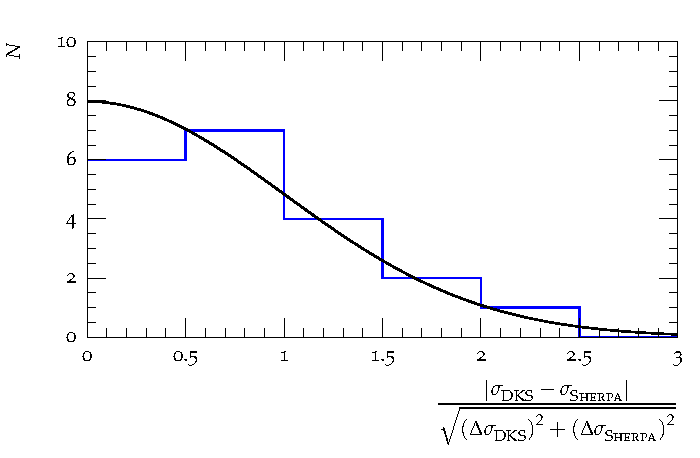
\includegraphics[width=0.5\textwidth]{comp-dist}
  \caption{
    Comparison of computed cross sections and relative 
    corrections of DKS and \Sherpa{}+\Recola. 
    For reference the black line 
    shows a properly normalised normal distribution.
    \label{fig:WWW:xscomp}
  }
\end{figure}


\subsection{Summary of salient features of WWW production
cross sections at NLO}

Having validated the NLO predictions for the integrated
cross sections of WWW production at the LHC, we briefly
summarize the salient features of the integrated and differential
cross sections based on the results presented in
Ref.~\cite{Dittmaier:2019twg}:

\begin{itemize}
\item
Similarly to the case of $\PW\PW\PW$ production with stable \PW bosons, 
a strong but accidental cancellation among the 
quark--antiquark and the remarkably large
quark--photon-induced EW corrections is observed.
For the chosen event setup at LHC energies of 13--14~TeV, 
they are of similar size ($\sim$\,7--8\,\%) but different in sign, 
so that the total EW corrections are below the percent level.
\item
QCD corrections at the LHC CM energies of 13--14\,TeV amount to approximately $40\,\%$.
As the analyzed process is independent of $\alpha_{\mathrm{s}}$ at LO, there is no decrease of the residual scale 
dependence from LO to NLO.
To obtain a reduction of the scale uncertainty, next-to-next-to-leading order (NNLO) QCD calculations 
or multi-jet merging would be necessary.
\item
Differential distributions show a strong impact of the EW high-energy logarithms, 
which reach 20--30\,\% in the TeV range.
Angular distributions are slightly modified in shape when including NLO corrections.
Thus, to constrain anomalous gauge couplings, the NLO corrections should be included.
\item
Apart from the full off-shell calculation, Ref.~\cite{Dittmaier:2019twg} presents results
on the NLO corrections to WWW production within a triple-pole approximation (TPA),
which is based on the leading term in the expansion of the one-loop matrix elements 
around the resonances of the three \PW bosons.
For a consistent comparison of TPA and fully off-shell results, the Higgs-strahlung subprocess
has to be excluded by phase space cuts,
which is possible due to the good separation originating from 
the small Higgs width and the mass hierarchy $M_{\PH}<2M_{\PW}$.
The TPA performs very well in integrated cross sections and in angular and rapidity distributions, 
which are insensitive to off-shell effects.
For some observables, however, that become sensitive to non-resonant contributions, 
like the missing transverse momentum at high scales, the TPA is not a sufficient approximation.
Sizable deviations can be observed in these regions.
Nevertheless, the size of the TPA uncertainty can be estimated reasonably well to identify 
those regions by analyzing TPA results only.
\end{itemize}
In summary, NLO results for EW corrections based on the full off-shell matrix elements 
are certainly sufficient for the analyses of WWW production at the LHC.
For integrated cross sections, even NLO EW corrections in the TPA will be sufficiently precise.


%= undefine macros (MANDATORY) ====================
\let\Herwig\undefined
\let\Pythia\undefined
\let\Sherpa\undefined
\let\Rivet\undefined
\let\Recola\undefined
\let\Professor\undefined
\let\Amegic\undefined
\let\OpenLoops\undefined
\let\Collier\undefined
\let\eps\undefined
\let\mc\undefined
\let\mr\undefined
\let\mb\undefined
\let\tm\undefined
\let\vp\undefined
\let\vP\undefined

